\setlength{\parindent}{0pt}

\clearpage
\section{Liveness DFA rules}
(Prepared by Jai Arora)
\vspace{0.3cm}

Now here we will define the transfer function for the Liveness Analysis. Define the function $L(s,x,in/out)$ as follows:

\begin{itemize}
    \item $x$ - the variable for which we want to compute the liveness values
    \item $s$ - a program statement $s$
    \item $in/out$ - whether it is input to the statement or output to the statement i.e just before the statement or just after the statement.
    \begin{itemize}
        \item $L(s, x, in)$ = The liveness value of $x$ just before s
        \item $L(s, x, out)$ = The liveness value of $x$ just after s i.e just after statement s is executed
    \end{itemize}
\end{itemize}

As discussed before, $L(s,x,in/out) \in \{{\tt true}, {\tt false}\}~\forall s,x$.\\

From now on, the discussion is for a particular variable $x$, but it can be generalized to more than one variables. We are going to define rules for the following 2 cases:

\begin{itemize}
    \item \textbf{Case 1:} A statement $p$ has one or more successor program points. So in this case, the $out$ value of the statement $p$ is expressed as a function of $in$ values of the successor program points.
    \begin{figure}[H]
        \centering
        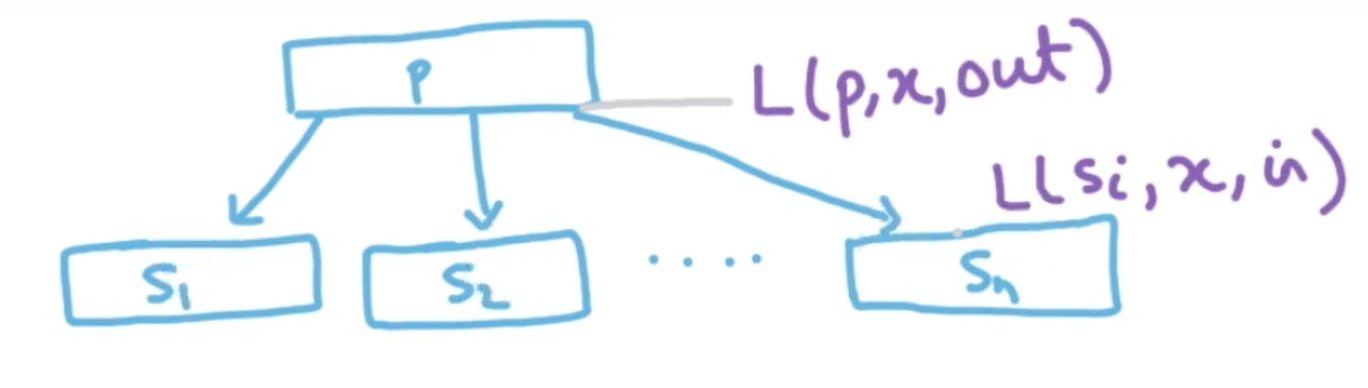
\includegraphics[height=3cm]{images/Module82_1.png}
    \end{figure}

    \item \textbf{Case 2:} For a given statement $s$, the $in$ value is a function of the $out$ value of that statement.
    \begin{figure}[H]
        \centering
        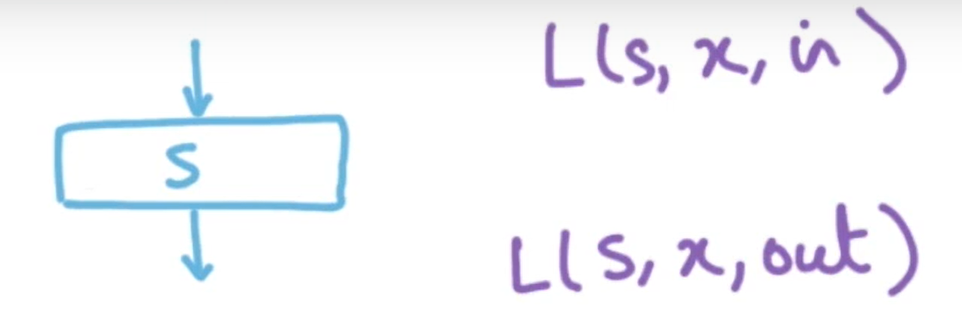
\includegraphics[height=3cm]{images/Module82_2.png}
    \end{figure}

\end{itemize}
It can be obseved from here that unlike Global Constant Propagation, which is a Forward Dataflow Analysis, this is a Backward Dataflow Analysis (it starts from the exit point).

\subsection{Rules for the Transfer Function:}
%Insert Images
\begin{itemize}
    \item $L(p, x, out) = glb\{L(s_i, x, in)~|~s_i$ is a successor of $p\}$\\
    
    If $x$ is live before any of the successors, then $x$ is live after that statement as it may get used in the downflow logic.
    \item If $s$ is of the form $... = f(...,x,...)$, then $$L(s, x, in) = {\tt true}$$ as the variable $x$ is getting used in this statement.
    \item If $s$ is of the form $x := e$, where $e$ is an expression which does not refer to $x$, then $$L(s, x, in) = {\tt false}$$ as we don't need the values of $x$ just above this statement due to $x$ being rewritten
    
    Note: If $e$ referred to $x$, then Rule \#2 would apply
    \item If $s$ does not refer to $x$ at all (neither updating it, nor using it), then $$L(s, x, in) = L(s, x, out)$$
\end{itemize}

These rules are exhaustive. These can be thought of as a system of equations, and our solution should satisfy all these rules.

\subsection{Liveness DFA Algorithm}
\begin{itemize}
    \item Initialize $L(s, x, in/out) = {\tt false}$ for all statements $s$ and variables $x$ (We start from a more aggresive value)
    \item Repeat until all program points satisfy Rules 1-4
    \begin{itemize}
        \item Pick a statement $s$ not satisfying one or more rules in rules 1-4 and update the corresponding $L()$ function value using the appropriate rule
    \end{itemize}
\end{itemize}

There is a guarantee that this algorithm will converge.